\documentclass{amsbook}
\usepackage{graphicx} % Required for inserting images
\usepackage[left=1.1cm,right=1.1cm,top=1.5cm,bottom=1.5cm]{geometry}%set margin of page
\usepackage{hyperref}
\usepackage{enumitem}
\usepackage{graphicx}
\usepackage{tikz}
\title{resume}
\author{Gerd Jana}
\date{September 2023}

\begin{document}

\begin{tikzpicture}[
    overlay,% Do our drawing on an overlay instead of inline
    remember picture,% Allow us to share coordinates with other drawings
    shift=(current page.north west),% Set the top (north) left (west) as the origin
    yscale=-1,% Switch the y-axis to increase down the page
]
    \clip (18,2) circle (1.5cm) node {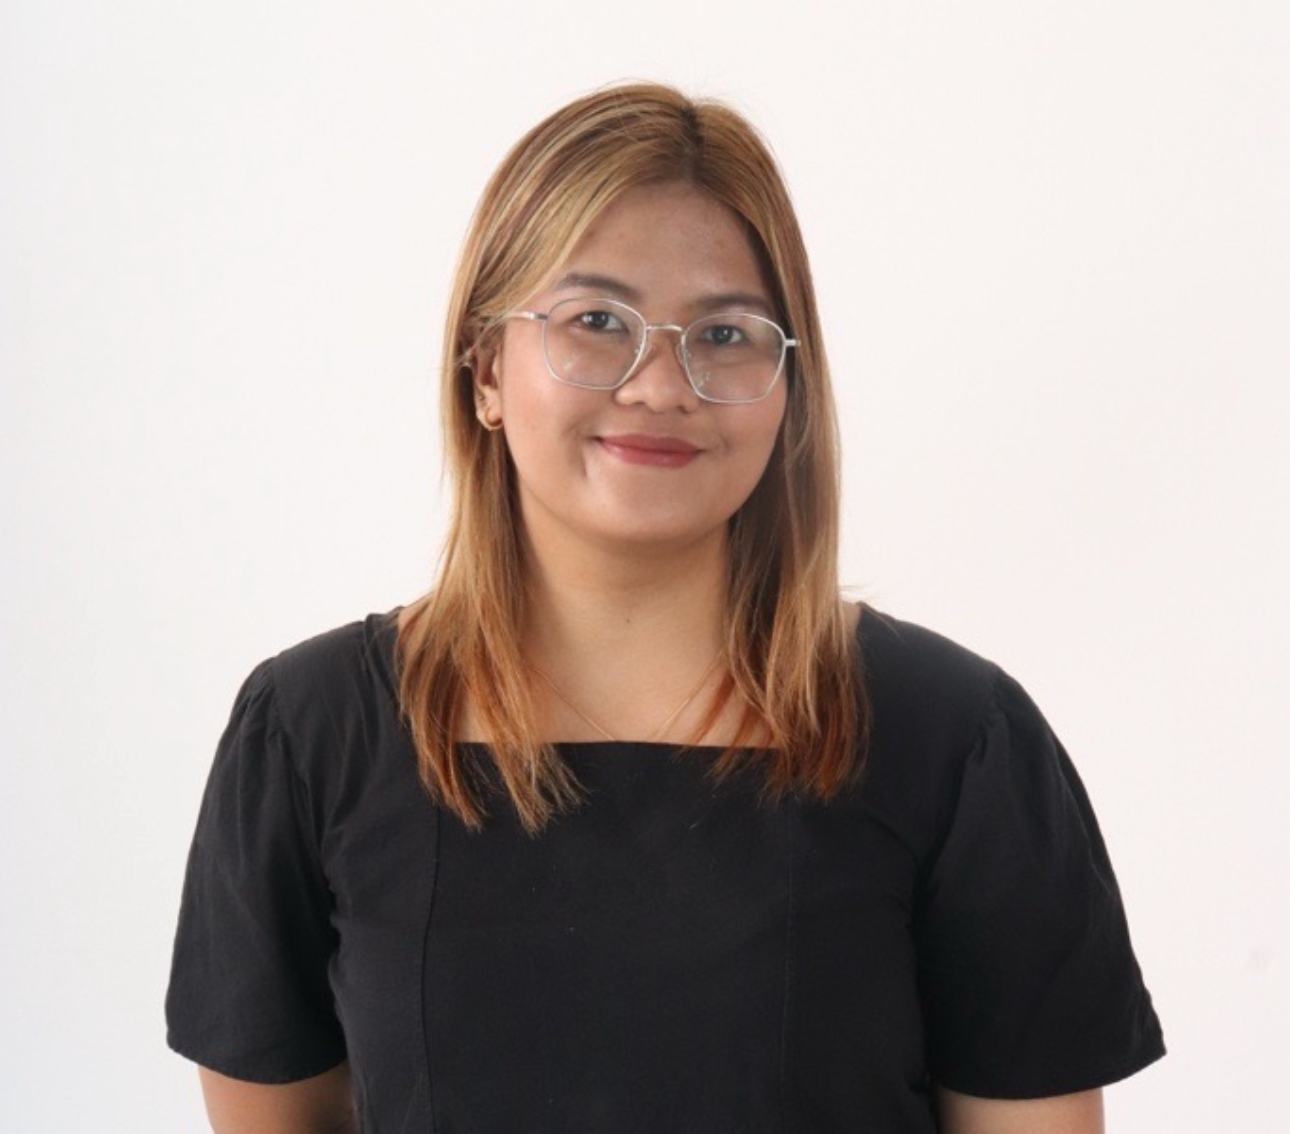
\includegraphics[width=4cm]{images/picture.jpg}};
    % \node at (7in, 1.2in) {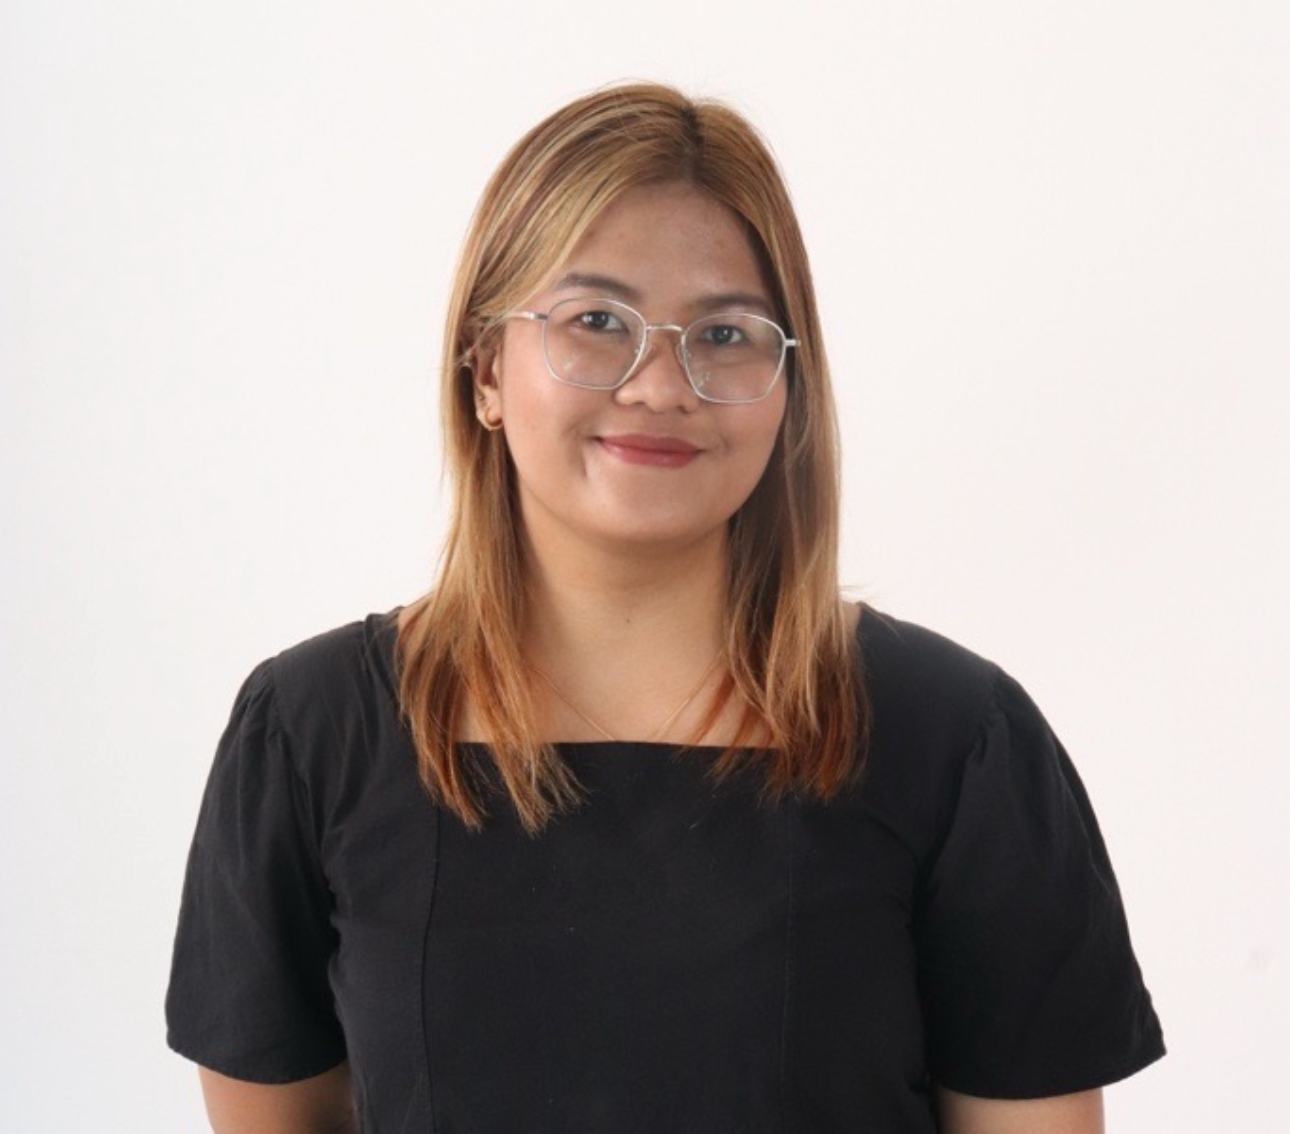
\includegraphics[width=1.5in]{images/picture.jpg}};
\end{tikzpicture}
\hspace{-1cm}\textbf{{\larger[8] Ericka Mae Bertes}}
\\\\
{\larger[2]\href{mailto:bertesericka@gmail.com}{bertesericka@gmail.com} } $|$ +63 (927) 022 1099 $|$ Naga City, Camarines Sur\\
\underline{\href{https://www.linkedin.com/in/ericka-mae-bertes-3590a2168/}{LinkedIn}} 
% $|$
% \underline{\href{https://github.com/gerdiedoo}{Github}} $|$
% \underline{\href{https://gerdiedoo.github.io/gerdjana/}{Website}}
\\
% \rule{\textwidth}{1pt} 
\\
\textbf{WORK EXPERIENCE}
\\
\rule{\textwidth}{1pt} 
\textbf{Associate Software QA Engineer \hfill Feb. 2022 \@- present}
\\
\textit{Navitaire Philippines Inc \hfill Taguig City}
\begin{itemize}
    \item Software tester of a web service and an application for revenue management
    \item Designs and executes test plans for functional, technical, and regression testing
    \item Executed performance testing of a web service using an automated script in C\# and Performance Monitor
    \item Designed and implemented automated test scripts using C\#
    \item Executed automated Gherkin and Specflow scripts for an automated test of an application
    \item Documents executed test plans and new features comprehensively
    \item Utilized Azure DevOps in reporting and tracking items and bugs
    \item Collaborates closely with an Agile Scrum Team consisting of backend developers and testers from design to retrospective
    
\end{itemize}
\noindent
\textbf{Software QA Tester Intern \hfill June 2021 \@- Aug. 2021}\\
\textit{Kitika Mobile Healthcare Inc \hfill Quezon City}
\begin{itemize}
    \item Assisted in detecting bugs in the website and mobile app.
    \item Tested  website and mobile apps and helped  in identifying deficiencies
    \item Assisted in testing the new website and mobile app versions through regression and stress testing and creating daily reports.
    \item Suggest solutions to identified problems.
    \item Using Agile Methodologies in the development.
    \item Creating test cases and executing them on the platform.
    \item Testing different phases of the app and website development
    \item Collaborate with the team in presenting bugs and giving ideas to solve the problems.
    \item Designed mockups for website and application
\end{itemize}
\noindent
\textbf{Naga City Youth Official \hfill April 2017 \@- March 2018}\\
\textit{Naga City Hall \hfill Naga City, CamSur}
\begin{itemize}
  \item Helped in developing programs for the youth
  \item Became the counterpart of Chief of Hospital of Naga City Hospital
  \item Helped in managing and organizing the events for Youth Month 2017 in Naga City
  
\end{itemize}
\noindent
\\
\textbf{EDUCATION}
\\
\rule{\textwidth}{1pt} 
\textbf{Bachelor of Science in Computer Engineering \hfill 2018 \@- 2022}\\
\textit{Ateneo de Naga University \hfill Naga City, CamSur}
\begin{itemize}
    \item Bachelor of Science in Computer Engineering
    \item Seniors' Project\@: Predicting Credibility of Filipino-Language Media with Natural Language Processing and Machine Learning (With a final rating of 98)
    \item General QPI\@: 3.25 (with 4.0 as the highest)  | With Honorable Mention
    \item Scholarships:
    \begin{itemize}
        \item College Scholarship Program
        \item Tanging Yaman Foundation Scholarship
    \end{itemize}
    
\end{itemize}
\noindent
\textbf{Camarines Sur National High School \hfill 2012 \@- 2018}\\
\textit{Science, Technology, Engineering, \& Mathematics \hfill Naga City, CamSur}
\begin{itemize}
    \item Graduated Senior High School in the Science, Technology, Engineering, and Mathematics track with High Honors and Outstanding Performance in Mathematics and Science
    \item Completed Junior High School in Science, Technology, and Engineering Curriculum with Honors
    
\end{itemize}
\noindent
\\\\\\\\\\
\textbf{AFFILIATIONS}
\\
\rule{\textwidth}{1pt} 
\noindent
\textbf{Institue of Computer Engineers in the Philippines Student Edition}
\textit{Bicol Chapter}
\begin{itemize}
    \item 2019\@-2020 President
    \item 2018\@-2019 Secretary
\end{itemize}
\noindent
\textbf{Computer Engineering Society}
\textit{Ateneo de Naga University}
\begin{itemize}
    \item 2021\@-2022 Auditor
    \item 2020\@-2021 President
    \item 2019\@-2020 External Vice President
    \item 2018\@-2019 Assistant Secretary
\end{itemize}
\noindent
\\
\textbf{AWARDS \& ACHIEVEMENTS}
\\
\rule{\textwidth}{1pt} 
\noindent
\textbf{Dean's Lister}
\begin{itemize}
    \item Second Semester, Academic Year 2021\@-2022
    \item First Semester, Academic Year 2018\@-2019
\end{itemize}
\textbf{National Programming Challenge Contestant}
\begin{itemize}
    \item Institute of Computer Engineers in the Philippines
    \item Citystate Asturias Hotel, Puerto Princesa, Palawan
    \item November 26\@-29, 2019
\end{itemize}
\textbf{Region V Programming Challenge Champion}
\begin{itemize}
    \item Institute of Computer Engineers in the Philippines Students Edition (Bicol Chapter)
    \item Ateneo de Naga University
    \item September 29, 2020
\end{itemize}
% \noindent
% \\\\
% \textbf{CERTIFICATIONS \& }
% \\
% \rule{\textwidth}{1pt} 
% \noindent
% \begin{itemize}[itemindent=-1cm]
%     \item \textbf{Certifications:}
%     \begin{itemize}[itemindent=-0.5cm]
%         \item Introduction to Packet Tracer $|$ \textit{Cisco Networking Academy $|$ 2020}
%         \item NDG Linux Unhatched Completion $|$ Cisco Networking Academy. $|$ \textit{2019}
%         \begin{itemize}[itemindent=-0.5cm]
%             \item NDG Linux Essentials
%             \item NDG Linux Series
%             \item IT Essentials
%         \end{itemize}
%     \end{itemize}
%     \item \textbf{Skills:} 
%     \begin{itemize}[itemindent=-0.5cm]
%         \item Can program in C, C++,  C\#, Java, and Python.
%         \item Can manage databases using MySQL\@.
%         \item Knowledgeable in using different Operating Systems \@- Linux (Ubuntu and Zorin OS),
%         \begin{itemize}[itemindent=-0.5cm]
%             \item[]Windows (XP/VISTA/7/8/8.1/10), and macOS\@. 
%         \end{itemize}
%         \item Has knowledge in MATLAB, Multisim Circuit Design Suite, PCB Wizard, and Eagle Layout.
%         \item Knowledgeable about basic concepts about Routing and Switching in CISCO Networking
%     \end{itemize}
% \end{itemize}
\noindent
\\
\textbf{CERTIFICATIONS}
\\
\rule{\textwidth}{1pt} 
\noindent
    \begin{itemize}
        \item Introduction to Packet Tracer $|$ \textit{Cisco Networking Academy $|$ 2020}
        \item NDG Linux Unhatched Completion $|$ Cisco Networking Academy. $|$ \textit{2019}
        \begin{itemize}
            \item NDG Linux Essentials
            \item NDG Linux Series
            \item IT Essentials
        \end{itemize}
    \end{itemize}
\noindent
\\
\textbf{SKILLS}
\\
\rule{\textwidth}{1pt} 
\noindent
\begin{itemize}
        \item Can program in C, C++,  C\#, Java, and Python.
        \item Can manage databases using MySQL\@.
        \item Knowledgeable in using different Operating Systems \@- Linux (Ubuntu and Zorin OS),
        \begin{itemize}[itemindent=-0.5cm]
            \item[]Windows (XP/VISTA/7/8/8.1/10), and macOS\@. 
        \end{itemize}
        \item Has knowledge in MATLAB, Multisim Circuit Design Suite, PCB Wizard, and Eagle Layout.
        \item Knowledgeable about basic concepts about Routing and Switching in CISCO Networking
\end{itemize}
\noindent
\\
\noindent
\\
\textbf{KEY STRENGTHS}
\\
\rule{\textwidth}{1pt} 
\noindent
\begin{itemize}
    \item Great communication and interpersonal skills
    \item Excellent organizational and administrative skills
    \item Can work in a team environment and independently
    \item Good problem-solving ability and analytical skills
    \item Excellent leadership skills
    \item Excellent at creating reports and presentations
    \item Fluent in English, Filipino, and Bikol
\end{itemize}
\noindent
\\\\
\end{document}
